
\newpage

    \subsection{Appendix 2 - Planning}
    \subsubsection{Gantt Chart}

    \begin{figure}[!ht]
    \centering
    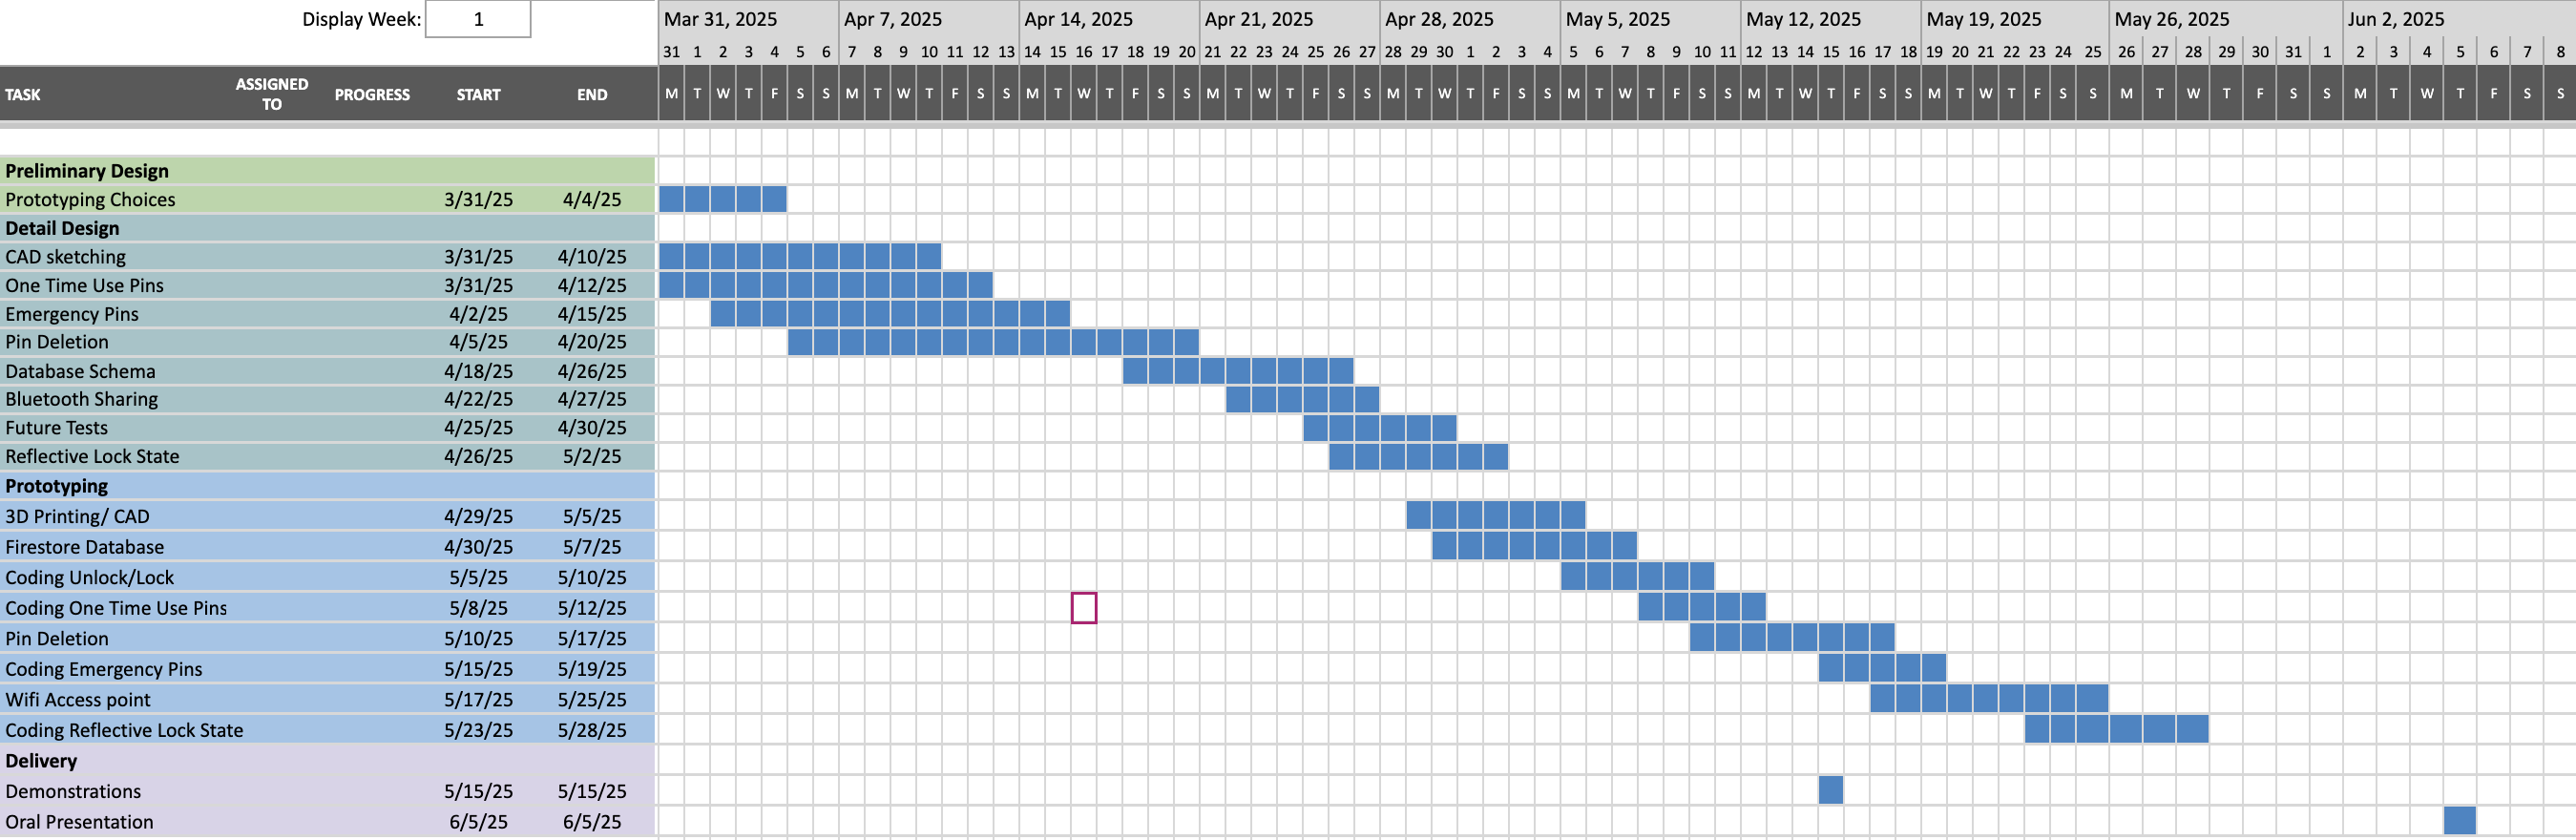
\includegraphics[width=0.80\textwidth]{img/ganttchart.png}
    \caption{Gantt Chart}
    \label{fig:ganttchart}
\end{figure}

\subsubsection{Division of Labor During Prototyping Phase}

Each team member contributed to different aspects of the system based on their strengths: \\

\textbf{Adam} focused on connectivity and user feedback through the hardware. He designed the Wi-Fi configuration process using an access point hosted by the ESP32-C3, allowing users to enter their network credentials during setup. He also implemented visual feedback through LEDs to indicate key system events like Wi-Fi disconnection and keypad input, which improved user interaction and made the system more transparent and intuitive. In addition to handling the microcontroller logic for reading and writing PIN codes, he also worked on sending acknowledgment signals to the database to reflect lock status. Adam read extensive documentation and shared his findings with the team, helping everyone better understand and use specific library functions needed for the embedded system. \\

\textbf{Jackson} handled mobile app development and the various components and package dependencies within it. Using Swift and Xcode, he built the app to support account creation, user authentication, locking and unlocking functions, and the generation of one time and emergency PINs. He implemented additional layers of security, including key protections for the emergency pins, and ensured the app could successfully interact with the Firestore database. This included writing data based on user actions as well as receiving values from the microcontroller. He focused on correctly storing, updating, and modifying values in response to user interactions, and handled database reads that reflected lock activity such as acknowledgement signals confirming a successful unlock. He made sure those values were then displayed in the app’s UI to keep the user informed of the lock’s state in real time. \\

\textbf{Nathaniel} worked on the embedded systems logic that connected keypad input to the solenoid lock’s behavior. He ensured the ESP32-C3 could correctly interpret keypad entries from the keypad and respond appropriately based on the type of PIN entered. He also developed the core functionality behind the one time PINs and emergency PINs, ensuring that they operated securely and reliably within different usage scenarios. In addition to his implementation work, Nathaniel designed and led many of the functional testing cases that helped us validate how the system responded to various edge cases, user actions, and failure conditions. He also contributed to the two-way acknowledgement system between the ESP32-C3 and Firestore, confirming that PIN entries were recognized and matched against those generated by the mobile application. \\

\textbf{Neena} focused on the physical and backend infrastructure of the project. Neena led the CAD design of the smart lock enclosure using Fusion 360, despite having no prior experience with CAD tools. Through tutorials, peer examples, and trial and error, she taught herself how to design for 3D printing and gradually refined the model over several iterations. Her final design featured a clean, minimal container with both top and bottom openings for easier assembly, accounted for hardware fit issues like oversized breadboards and solenoid lock dimensions, and included a small window to make the LED indicators visible from outside. Neena also took charge of defining the Firestore database schema. The system initially supported a basic one-to-many relationship where one user could access multiple locks, but Neena recognized that this would be too limiting for real world use cases. She advocated for and designed a more flexible many-to-many model, allowing multiple users to share access to multiple locks. This included structuring user and lock collections separately, and introducing a join collection to manage shared permissions and access levels. While the full implementation of this schema wasn’t completed due to time constraints, her planning laid a foundation for scaling the access control logic in future versions of the product. \\

All members contributed to system integration, documentation, poster/presentation design, and final testing.

\subsubsection{Collaboration}

We worked closely as a team throughout the entire project, meeting regularly both in person and over Discord. In person sessions were especially helpful when it came to debugging, assembling the prototype, and running tests, while Discord helped us stay connected between meetings and keep progress moving asynchronously. \\

We used GitHub to manage version control, pushing and reviewing code through pull requests and keeping our work organized across different components. While we each focused on our own areas like app development, CAD, or firmware, we were always checking in with each other, helping troubleshoot bugs, and making decisions together when things didn’t go as expected. \\

We also utilized the Arduino IDE for the ESP32-C3 firmware, which allowed us to share code snippets and collaborate on the microcontroller logic. This was particularly useful for integrating the keypad input with the solenoid lock and ensuring that the Firestore database updates were correctly reflected in the mobile app. We used the Arduino IDE because it contained all the libraries needed for firestore and ESP32-C3 development. \\

As we got closer to the deadline, collaboration became even more hands on. We met frequently to run hardware tests, make final tweaks to the CAD design, rehearse the demo, and wrap up our documentation and poster. Even though we had separate roles, we shared a strong sense of team ownership, which helped keep the project on track and made the experience feel really rewarding. \\
